% !TEX root = ../spec_kernel_agent_main.tex
\section{Methodology}\label{sec:design}

This section details the two components of \sysname{}: \emph{SpecController} (\S\ref{subsec:speclauncher}), which decides when and how to fork speculative generations, and \emph{ElasticScheduler} (\S\ref{subsec:asyncscheduler}), which dynamically resizes the resource pool and orchestrates concurrent validation and profiling requests.

\begin{figure}[t]
    \centering
    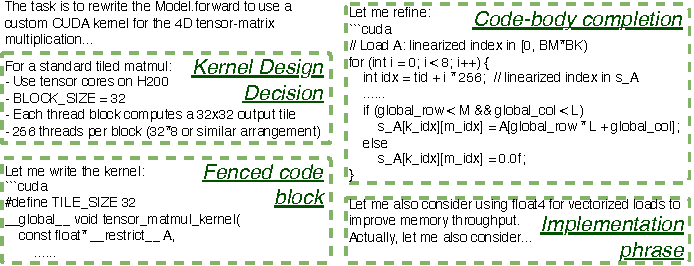
\includegraphics[width=\linewidth]{figs/kerneldesignintrace.pdf}
    \vspace{-20pt}
    \caption{A reasoning trace of GLM-5.1 on the 4D tensor Matmul task. Trigger signals are highlighted in red.}
    \label{fig:kerneldesignintrace}
    \vspace{-15pt}
\end{figure}
\subsection{SpecController}\label{subsec:speclauncher}

Algorithm~\ref{alg:speclauncher} shows when SpecController forks speculative generations and when it 
terminates the reasoning generation.
SpecController monitors the reasoning generation's output. At selected trigger points, 
it concatenates this iteration's prompt with the reasoning prefix to form a speculative prompt.
Conditioned on this speculative prompt, SpecController forks non-reasoning generations 
and dispatches their emitted kernels to validation and profiling while the reasoning generation 
continues as a fallback.
Once a kernel meets the termination criterion, SpecController terminates the reasoning generation
and all pending speculative generations to reduce generation latency.
We next detail when SpecController triggers speculative generations~(\S\ref{subsubsec:dynparser}) and when it terminates the reasoning generation~(\S\ref{subsubsec:dispatch}).

\begin{algorithm}[t]
\caption{SpecController core loop.}
\label{alg:speclauncher}
\begin{algorithmic}[1]
\Require Reasoning LLM $M$, prompt $P_0$, search algorithm $\mathcal{A}$, resource capacity $C$, \#iterations $N$
\State $H \gets \{0\}$;\, $P \gets P_0$ \Comment{Speedup history; initial prompt}
\State $k^{\star} \gets \bot$ \Comment{Best kernel found so far}
\For{$i = 1$ \textbf{to} $N$}
    \State $et \gets \textbf{false}$ \Comment{Early termination flag}
    \State $\mathcal{G} \gets$ stream of $M(P)$ \Comment{Reasoning generation}
    \While{$\mathcal{G}$ is not terminated}
        \If{$\mathcal{G}$ emits a trigger signal \textbf{or} GPU is idle}
            \State $\pi \gets$ prefix of $\mathcal{G}$
            \State $P_s \gets CONCAT(P, \pi)$ \Comment{Speculative prompt}
            \State $K \gets \max(1, \min(C.\textit{val}, C.\textit{prof}))$ \label{line:num_spec_gens}
            \State Fork $K$ spec. generations with prompt $P_s$.
        \EndIf
        \For{each spec. generation $G_s$ with kernel $k_s$}
            \State $speedup_s \gets$ measured speedup of $k_s$
            \State $\tau \gets \mathrm{mean}(H)$
            \State $H \gets H \cup \{speedup_s\}$
            \If{$speedup_s > \tau$}
                \State $k^{\star} \gets k_s$; \, $et \gets \textbf{true}$
                \State Terminate $\mathcal{G}$ and all pending forks;
                \State \textbf{break}
            \EndIf
        \EndFor
    \EndWhile
    \If{$et$ is \textbf{false}}
        \State Update $k^{\star}$ with the best found kernel.
    \EndIf
    \State $P \gets \mathcal{A}(k^{\star},\, H)$ \Comment{Update prompt for next iteration}
\EndFor

\State \Return $k^{\star}$ \Comment{The best found kernel}

\end{algorithmic}
\end{algorithm}

\subsubsection{Trigger Speculative Generation}\label{subsubsec:dynparser}
SpecController uses kernel-design decisions in the reasoning trace as trigger
signals for speculative generations.
Figure~\ref{fig:kerneldesignintrace} shows an example of the reasoning trace from GLM-5.1 on the 4D tensor Matmul task.
During the reasoning process, we observe that the LLM commits concrete
kernel-design decisions.
As reasoning progresses, the LLM implements these decisions in fenced code
blocks or completed kernel bodies.
Finally, the LLM generates the final code based on the reasoning results.
Based on this observation, SpecController uses an empirical parser to detect
these trigger signals.
The parser recognizes four classes of trigger signals.
(1) \emph{Kernel-design decisions.} Concrete kernel-design decisions, such as tile shapes, tile sizes, and specific instructions.
(2) \emph{Fenced code blocks.} Complete code blocks fenced with language tags such as \texttt{cuda}, \texttt{cpp}, or \texttt{python}.
(3) \emph{Kernel-body completion.} A partial kernel body, such as a \texttt{\_\_global\_\_} function with a complete
signature and brace-balanced body.
(4) \emph{Implementation phrases.} Natural-language phrases that announce implementation, such as ``Let me implement\ldots'', ``Here is the plan\ldots''.
We derive these trigger structures from 38{,}745 reasoning traces generated by
GLM-5.1 and DeepSeek-V4-Pro, and implement the parser with regular expressions.

Once SpecController detects these trigger signals, 
it concatenates the iteration's original prompt and the reasoning trace
prefix to construct a speculative prompt.
Then SpecController forks non-reasoning generations with this speculative prompt.
To avoid speculative-generation starvation when no trigger is detected,
SpecController also forks from the current reasoning prefix whenever
validation/profiling resources become idle.
Each fork event launches $K$ speculative generations, where $K$ is determined by 
the resource capacity $C$ (Algorithm~\ref{alg:speclauncher}, Line~\ref{line:num_spec_gens}).
This lets SpecController launch enough speculative generations to keep resources
busy without queuing too many requests and wasting tokens.

\subsubsection{Early Termination}\label{subsubsec:dispatch}
SpecController terminates the reasoning generation once a speculative
kernel meets the predefined termination criterion.
After a speculative generation emits a candidate kernel, SpecController sends it
to ElasticScheduler (\S\ref{subsec:asyncscheduler}) for validation and profiling.
For each valid kernel, ElasticScheduler returns the measured speedup over the
\texttt{KernelBench} reference.
SpecController maintains a history $H$ of previously profiled kernel speedups
and compares each new kernel's speedup against this history.

\begin{figure}[t]
    \centering
    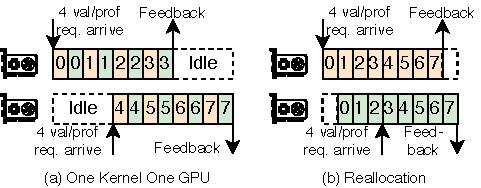
\includegraphics[width=\linewidth]{figs/asyncscheduler.pdf}
    \vspace{-20pt}
    \caption{Reducing GPU idle with reallocation.}
    \label{fig:asyncscheduler_workflow}
    \vspace{-15pt}
\end{figure}
In our experiments, we use the mean speedup of previously profiled kernels, $\mathrm{mean}(H)$, as
the termination threshold. When a speculative kernel exceeds this threshold, 
SpecController terminates the reasoning generation and cancels all pending
speculative generations. Otherwise, the reasoning generation continues as a fallback.
This adaptive threshold maintains termination frequency without sacrificing kernel performance.
Figure~\ref{fig:token_kernel_speedups_GLM_5_1} empirically confirms the efficiency of this termination criterion.
As optimization progresses, $\mathrm{mean}(H)$ rises with the performance of previously found kernels.
At the same time, it is less sensitive than $\max(H)$ to a 
single outlier, which could otherwise suppress early termination for many later iterations.
For example, on the Diagonal Matmul task, a kernel reaches
56$\times$ speedup over the reference in iteration 5 and remains the best kernel until iteration 72 (Figure~\ref{fig:token_kernel_speedups_GLM_5_1}).
If the threshold were $\max(H)$, early termination would rarely fire during this
interval, losing generation-latency savings without improving the best kernel.
Instead, using $\mathrm{mean}(H)$ as the threshold allows SpecController to
reduce generation latency through more frequent early termination
(Figure~\ref{fig:e2e_execution_time}).
\sysname{} also exposes interfaces for user-supplied termination criteria.


\algnewcommand\algorithmicasync{\textbf{async}}
\algdef{SE}[ASYNC]{Async}{EndAsync}
{\algorithmicasync}
{\algorithmicend\ \algorithmicasync}

\begin{algorithm}[t]
\caption{ElasticScheduler core loop.}
\label{alg:asyncscheduler}
\begin{algorithmic}[1]
\Require Total GPU pool $G$
\State $Q_v \gets \emptyset$;\, $Q_p \gets \emptyset$ \Comment{Request queues}
\State $L_v \gets 0$;\, $L_p \gets 0$ \Comment{Max queue lengths}
  \For{each iteration $i$}
      \State $(G_{val}, G_{prof}) \gets \Call{Allocate}{L_v, L_p, G}$ \Comment{Reallocation}
      \State $L_v \gets 0$;\, $L_p \gets 0$ \Comment{Reset max queue lengths}
      \Async
      \State Queue requests to $Q_v$ (LAF) and $Q_p$ (FIFO).
      \State $L_v \gets \max(L_v, |Q_v|)$;\, $L_p \gets \max(L_p, |Q_p|)$
      \State Serve requests with $G_{val}$ and $G_{prof}$ on idle GPUs.
      \EndAsync
      \State Terminate in-flight requests and clear $Q_v$ and $Q_p$.
  \EndFor
\end{algorithmic}
\end{algorithm}
\subsection{ElasticScheduler}\label{subsec:asyncscheduler}

Algorithm~\ref{alg:asyncscheduler} illustrates the core loop of ElasticScheduler.
At the beginning of each iteration, ElasticScheduler calls \Call{Allocate}{} to reallocate the validation/profiling GPU split
$(G_v, G_p)$ based on the maximum validation and profiling queue lengths, $L_v$ and $L_p$, from the previous iteration.
ElasticScheduler receives validation and profiling requests from SpecController and serves them on the corresponding GPU split with two priority queues.
At the iteration boundary, SpecController consumes only the validation/profiling
results that have already returned.
ElasticScheduler then aborts remaining requests from the finished iteration and
clears both queues, so speculative tails never delay the next iteration.
Finally, ElasticScheduler repurposes unused GPU memory in the validation/profiling
GPUs as remote KV-cache storage for the reasoning prefix.
We next detail the resource reallocation (\S\ref{subsubsec:priqueue}), the priority queues (\S\ref{subsubsec:reduce_prof_latency}), and the remote
cache of reasoning prefixes (\S\ref{subsubsec:remote_cache}).

\subsubsection{Resource Reallocation}\label{subsubsec:priqueue}

ElasticScheduler divides the total GPU pool into two splits: validation GPUs and profiling GPUs.
The number of GPUs in each split is determined by the max queue length $L_v$ and $L_p$ from the previous iteration.
Specifically, when $L_v + L_p = 0$, ElasticScheduler uses an even split.
Otherwise, it sets $G_{prof} = \min(G-1, \max(1, \left\lceil G \cdot \frac{L_p}{L_v + L_p} \right\rceil)), 
\quad G_{val} = G - G_{prof}$.
With this reallocation, ElasticScheduler can absorb bursty speculative-generation load and reduce GPU idle.
Figure~\ref{fig:asyncscheduler_workflow} shows an example of the resource reallocation.
In this example, the static one-GPU-per-phase allocation keeps one GPU assigned
to validation and one GPU assigned to profiling.
Because validation and profiling requests arrive at different times, one split
can queue requests while the other split remains idle.
ElasticScheduler reallocates the two GPUs according to the previous iteration's
queue pressure, allowing idle GPUs to move toward the heavier-loaded phase.


\subsubsection{Reducing Profiling Feedback Latency}\label{subsubsec:reduce_prof_latency}

ElasticScheduler prioritizes latest-arrival validation requests (LAF) and
earliest-arrival profiling requests (FIFO).
Later validation requests are produced from longer reasoning prefixes.
They are therefore conditioned on more design information than earlier requests.
Later candidates are therefore more likely to contain complete design
information and to meet the early-termination threshold.
LAF intentionally favors fresher candidates within an iteration.
Older validation requests may be skipped at the iteration boundary, but this does
not block progress because the reasoning generation remains a fallback and
the next iteration starts with a cleared queue.
For profiling requests, FIFO avoids delaying an already validated kernel behind
later arrivals.
Because every profiled kernel provides usable feedback, serving the oldest
validated kernel first reduces feedback latency without favoring speculative
freshness.

\subsubsection{Remote Cache of Reasoning Prefixes}\label{subsubsec:remote_cache}

Speculative generations share the reasoning prefix with the main generation.
However, keeping all prefix KV caches in local serving memory can exceed the
memory budget when multiple speculative generations are active.
ElasticScheduler therefore uses spare memory on validation/profiling GPUs as
remote KV-cache storage.
Validation and profiling consume little GPU memory in our workload, even under
bursty speculative load, so the remote cache uses otherwise idle memory without
reducing the memory available to validation or profiling execution.

When local serving memory approaches its capacity limit, ElasticScheduler
migrates KV caches of suspended reasoning prefixes to the remote GPU pool
instead of discarding them.
When a speculative generation later resumes from the same prefix, it restores
the cached KV state rather than recomputing the prefix from tokens~\cite{vLLM}.
The migration uses the Mooncake~\cite{Mooncake} backend for high-throughput device-to-device
RDMA transfers, avoiding the CPU/TCP data path.
This reduces prefix recomputation under a limited memory budget, further improving the system efficiency (see \S\ref{subsec:eval_performance_breakdown}).

\section{Implementation}\label{subsec:impl}

\sysname{} is implemented in approximately 9k lines of Python code.
SpecController monitors the LLM's reasoning trace through the OpenAI API v2.16.0.
SpecController parses the reasoning trace to detect trigger signals with a regular expression parser built on 38{,}745 reasoning traces from GLM-5.1 and DeepSeek-V4-Pro.
ElasticScheduler runs as a microservice to manage the validation and profiling requests.
Validation workers compile each candidate kernel via \texttt{nvcc} driven by Ninja 1.13.0 with \texttt{MAX\_JOBS=20}, then run a single correctness check against the \texttt{KernelBench} reference on the validation GPU.
Profiling workers invoke NCU 2025.1.0 for hardware-counter collection. Both validation and profiling workers run exclusively on GPUs.
The system exposes interfaces for user-defined search algorithms, prompt templates, and termination criteria.